\documentclass[sigconf]{acmart}

% DREAM II SIGCITE LaTeX export
% Camera-ready identity setting:
\newif\ifanonymousreview
\anonymousreviewfalse
% Set to \anonymousreviewtrue only for a future anonymized review copy.

\usepackage{booktabs}
\usepackage{array}
\usepackage{tikz}
\usetikzlibrary{arrows.meta,positioning,shapes.geometric}
\usepackage{enumitem}
\setlist{nosep,leftmargin=*}

\AtBeginDocument{%
  \providecommand\BibTeX{{Bib\TeX}}}

\copyrightyear{2026}
\acmYear{2026}
\setcopyright{cc}
\setcctype{by}
\acmConference[SIGCITE '26]{27th Annual ACM Conference on Cybersecurity and Information Technology Education}{November 12--14, 2026}{Wilmington, NC, USA}
\acmBooktitle{27th Annual ACM Conference on Cybersecurity and Information Technology Education (SIGCITE '26), November 12--14, 2026, Wilmington, NC, USA}
\acmDOI{10.1145/3857770.3858231}
\acmISBN{979-8-4007-3084-9/2026/11}

\title{Prompt Fidelity in LLM-Assisted Assessment: Rubric Drift and Operational Validation of an AI-Resilient Cybersecurity Assessment Rubric}

\ifanonymousreview
\author{Anonymous Author(s)}
\affiliation{\institution{Anonymous Institution}\country{Anonymous}}
\else
\author{Jennifer McCauley}
\affiliation{\institution{The Pennsylvania State University}\department{College of Information Sciences and Technology}\city{University Park}\state{PA}\country{USA}}
\email{jcw173@psu.edu}

\author{Edward J. Glantz}
\affiliation{\institution{The Pennsylvania State University}\department{College of Information Sciences and Technology}\city{University Park}\state{PA}\country{USA}}
\email{ejg8@psu.edu}

\author{Mahdi Nasereddin}
\affiliation{\institution{The Pennsylvania State University--Berks}\department{College of Information Sciences and Technology}\city{Reading}\state{PA}\country{USA}}
\email{mxn16@psu.edu}

\author{Michael R. Bartolacci}
\affiliation{\institution{The Pennsylvania State University--Berks}\department{College of Information Sciences and Technology}\city{Reading}\state{PA}\country{USA}}
\email{mrb24@psu.edu}
\fi

\begin{abstract}
Frameworks for generative-AI-resilient assessment have proliferated faster than their empirical validation. When a large language model (LLM) applies a rubric, reliability and validity are meaningful only if the model first executes the specified protocol. We define prompt fidelity as sustained adherence to the complete instructional intent of an evaluation prompt, and report rubric drift, an observed failure in which an LLM silently substituted a coherent but different five-dimension framework for the published instrument. Drift of this kind is routinely experienced, and tolerated, in everyday LLM use; in rubric-based assessment it invalidates every downstream statistic and must be prevented by overt prompt design. After detecting the substitution before statistical analysis, we repaired and froze the evaluator prompt by embedding the complete rubric, prohibiting criterion substitution, requiring anchor-cited rationales, and verifying the dimension set before and during scoring. Four cybersecurity faculty and the corrected LLM independently evaluated 10 public cybersecurity assignment prompts with a published five-dimension rubric. Over the four dimensions with score variation, faculty-faculty agreement was fair to moderate (mean Gwet AC1 = 0.287; mean quadratic weighted kappa = 0.408); including the provenance-floored Ethical GenAI Use dimension inflates these values to 0.451 and 0.485. Corrected LLM-faculty agreement was comparable (four-dimension mean AC1 = 0.216 and kappa = 0.474; five-dimension basis AC1 = 0.388 and kappa = 0.573). Ethical GenAI Use showed a complete floor effect attributable to sample provenance: all sampled prompts predated explicit classroom GenAI disclosure expectations. The results support cautious use of a prompt-faithful LLM as one disclosed input to assignment triage, not as a replacement for faculty judgment. The principal contribution is methodological: prompt fidelity must be verified before agreement statistics or validity claims are interpreted.
\end{abstract}

\keywords{prompt fidelity, rubric drift, LLM-as-judge, AI-resilient assessment, cybersecurity education, inter-rater agreement, Gwet AC1}

\begin{CCSXML}
<ccs2012>
 <concept>
  <concept_id>10003456.10003457.10003527.10003531</concept_id>
  <concept_desc>Social and professional topics~Student assessment</concept_desc>
  <concept_significance>500</concept_significance>
 </concept>
 <concept>
  <concept_id>10002978.10003006</concept_id>
  <concept_desc>Security and privacy</concept_desc>
  <concept_significance>300</concept_significance>
 </concept>
 <concept>
  <concept_id>10010147.10010178.10010179</concept_id>
  <concept_desc>Computing methodologies~Natural language processing</concept_desc>
  <concept_significance>300</concept_significance>
 </concept>
</ccs2012>
\end{CCSXML}
\ccsdesc[500]{Social and professional topics~Student assessment}
\ccsdesc[300]{Security and privacy}
\ccsdesc[300]{Computing methodologies~Natural language processing}

\begin{document}
\maketitle

\section{Introduction}
Generative AI has changed the evidentiary value of common written assessments. A plausible incident report, policy memo, configuration explanation, or case analysis can now be produced with limited student engagement, so assessment design must elicit situated performance, visible process, verification, and evaluative judgment rather than merely polished prose \cite{miao2023guidance,powell2024generative}. Cybersecurity is especially exposed because its assignments often combine technical artifacts with explanatory writing, both of which can be partially outsourced to generative systems.

A growing literature therefore treats LLMs as evaluators as well as producers. LLM-as-judge methods can score, rank, or critique outputs at scale, and evidence-anchored prompting can improve alignment with human judgment \cite{liu2023geval,zheng2023judging}. Yet these methods introduce a prerequisite that conventional reliability studies can usually take for granted: the evaluator must be applying the intended instrument. A fluent LLM can appear procedurally compliant while omitting, reinterpreting, or replacing core criteria \cite{thakur2025judging}.

We call sustained execution of the full evaluation protocol \emph{prompt fidelity}. The construct concerns whether the model performs the task that was specified, not whether its scores agree with a human rater or support a valid inference. Reliability asks whether raters agree. Validity asks whether the resulting scores support their intended use \cite{messick1995validity}. Prompt fidelity precedes both, because agreement computed on a substituted rubric is not low-quality evidence about the intended instrument; it is evidence about a different task. This ordering, fidelity, then reliability, then validity, structures the entire study.

McCauley et al. \cite{mccauley2025undergraduate} introduced a formative rubric for redesigning undergraduate cybersecurity assignments in the GenAI era. Its five dimensions are Authenticity, Process Transparency, Ethical GenAI Use, Interactive Verification, and Evaluative Judgment, each scored from 1 (not addressed) to 3 (fully addressed). The original paper positioned the rubric as a practical design diagnostic and explicitly deferred empirical validation. The present study extends that program and examines operational consistency before later construct validation.

The planned pilot compared independent faculty ratings with ratings from a frozen LLM evaluator. During prompt testing, however, the LLM repeatedly departed from the published dimensions, in the most complete instance replacing them wholesale with a new framework while preserving the expected output format. Because totals and threshold decisions still appeared reasonable, only a direct inspection of dimension names exposed the failure. We term this failure \emph{rubric drift} and document the fully developed episode in Section~\ref{sec:drift}.

Experienced LLM users encounter and routinely tolerate drift of this kind in everyday use. Rubric-based assessment cannot tolerate it: a drifted evaluator produces statistics about an instrument nobody intended to administer, so drift must be prevented and detected by overt prompt design rather than left to user forbearance. The event changed the study from a straightforward agreement pilot into a methodological demonstration of why prompt fidelity must be verified at runtime.

The study asks: RQ1, can four cybersecurity faculty apply the published rubric with useful agreement? RQ2, after prompt fidelity is verified, how closely does an LLM evaluator agree with faculty? RQ3, how stable is the rubric's redesign decision at the published threshold? RQ4, what procedural safeguards are required to prevent or detect rubric drift? We contribute a clarified construct hierarchy, a documented drift case, a repair workflow, and pilot agreement estimates that inform a larger external validation.

\section{Related Work}
\subsection{AI-resilient assessment}
AI-resilient assessment shifts attention from prohibiting tools to designing performances for which authorship, process, and judgment remain visible. Recommended strategies include authentic contexts, staged work, reflection on tool use, live or interactive verification, and critique of alternatives \cite{akbar2025beyond,fowler2023ai,jongkind2026curriculum,mccauley2025undergraduate}. These strategies align with established authentic-assessment and rubric traditions, which emphasize explicit criteria and evidence-based judgments rather than surface completion alone \cite{rhodes2013value}. The present study evaluates prompt design, not student performance, so it provides operational evidence about the instrument but not yet evidence that high-scoring prompts produce more AI-resilient learning outcomes.

\subsection{LLM-as-judge}
LLM-as-judge research shows that language models can approximate human evaluators in structured settings, but can also exhibit positional, verbosity, self-preference, and prompt-sensitivity biases \cite{liu2023geval,thakur2025judging,zheng2023judging}. Accordingly, model scores require transparent prompts, anchored rationales, reproducible artifacts, and comparison with human judgments. Human-centered AI further argues for designs in which automation augments rather than obscures accountable professional judgment \cite{shneiderman2022human}.

\subsection{Prompt fidelity and rubric instability}
Four related terms require separation. Prompt fidelity is session-level adherence to the complete requested evaluation protocol. Rubric drift is the observable failure documented here: wholesale substitution of criteria while the output retains a compliant appearance. Rubric instability describes inference-time changes in interpretation or scoring under a nominally fixed rubric, a focus of concurrent locked-rubric work \cite{hong2026rubrics}. Intent fidelity concerns whether individual dimensions preserve the user's intended meaning under structured prompt changes \cite{peng2026dimension}. Our contribution is not priority over these concurrent formulations, but an educational-assessment operationalization in which fidelity is checked before reliability is calculated. Prompt fidelity is therefore narrower than general instruction following and distinct from evaluator consistency or reproducibility: it asks whether the specified evaluation protocol remained intact during a scoring session, whereas consistency and reproducibility ask whether repeated applications produce comparable judgments.

\subsection{Reliability and operational validation}
Rubric studies commonly use chance-corrected agreement measures, but kappa can be depressed when one category dominates despite high observed agreement \cite{feinstein1990high}, a miscalculation risk documented in practice with the AAC\&U VALUE rubrics \cite{szafran2017miscalculation}. Gwet AC1 is less sensitive to this prevalence problem and was selected as the primary statistic, with quadratic weighted kappa retained because the rubric categories are ordinal \cite{cohen1968weighted,gwet2008computing}. In practical terms, AC1 estimates chance-corrected rater agreement while remaining less sensitive than kappa to highly concentrated score distributions; quadratic weighted kappa additionally gives greater credit to near agreement on the rubric's ordered 1-to-3 scale. Bootstrap resampling provides an empirical estimate of uncertainty around these agreement statistics. Operational validation in this paper means consistency of rubric application and decision behavior. It does not establish the broader validity argument envisioned by Messick \cite{messick1995validity}, which requires evidence about consequences, generalization, and the relationship between prompt scores and student performance.

\section{Methods}
\subsection{Study Design}
This was a pilot operational-validation study using only publicly available instructional materials. Four cybersecurity faculty investigators independently applied the published rubric, and a frozen LLM evaluator independently scored the same analytic sample. Faculty judgments were not treated as an infallible gold standard; instead, the design compared agreement among faculty and between each faculty rater and the model. The analysis used publicly available assignment prompts and author-generated rubric ratings; it involved no student records, student work, interviews, surveys, or individual-level outcomes. The published redesign threshold was retained: total scores below 10 of 15 indicate REVISE, while scores of 10 or above indicate KEEP. A spreadsheet label that stated ``10 and below'' was identified after scoring as an implementation error and was not used as the study's analytic threshold.

\begin{table}[t]
\caption{Study design summary.}
\label{tab:design}
\begin{tabular}{@{}p{0.34\linewidth}p{0.58\linewidth}@{}}
\toprule
Component & Specification \\
\midrule
Faculty raters & 4 cybersecurity faculty investigators \\
Assignment prompts & 10 public prompts \\
Sources & CLARK (9) and SEED Labs (1) \\
Unit of analysis & One assignment = one prompt = one artifact \\
LLM evaluator & Frozen institutional-platform session; temperature 0 and zero retention requested \\
Primary statistic & Gwet AC1 \\
Secondary statistic & Quadratic weighted kappa \\
Uncertainty & 1,000-resample bootstrap 95\% CIs \\
Published threshold & Total $<$ 10 = REVISE; total $\geq$ 10 = KEEP \\
\bottomrule
\end{tabular}
\end{table}

\subsection{Assignment Sample}
The sample contained 10 assignment prompts selected to vary by course level and task form: two introductory, four intermediate, two capstone, one graduate, and one advanced-undergraduate assignment. Five forms were represented: applied case or project, lab scenario, written deliverable, policy or design outline, and tool-based mapping. Nine prompts came from the CLARK Cybersecurity Curriculum Library and one from SEED Labs. Eight were licensed CC BY-NC-SA 4.0, one CC BY 4.0, and one was a U.S. government work in the public domain. Because the noncommercial and share-alike terms are not compatible with verbatim ACM reproduction, the paper reports prompt properties and source links rather than full text.

The prompts were scored as originally published. All 10 predated explicit classroom GenAI disclosure and justification requirements, so a score of 1 on Ethical GenAI Use was expected a priori unless such language had later been retrofitted. This historical feature was treated as sample provenance, not as evidence of deficient assignment quality: a uniform floor on this dimension reflects when the assignments were written and provides no evidence about rater inconsistency or about the dimension's ability to discriminate among contemporary assignments. The unit of analysis was fixed as one assignment, one prompt, and one scorable artifact.

\subsection{Faculty Calibration}
Before analytic scoring, the four investigators reviewed the published dimension definitions and anchors, applied the rubric to a calibration prompt outside the sample, and discussed criterion interpretation without establishing a forced consensus score. Each rater then scored all 10 prompts independently and supplied a one-sentence, prompt-specific rationale for every dimension. Scores were entered on separate workbook tabs. Because faculty scored asynchronously in a shared workbook, presentation order was held constant for them rather than randomized; this design limitation is addressed in Section~\ref{sec:limitations}.

\subsection{Prompt-Faithful LLM Evaluator}
The initial evaluator prompt referenced the rubric indirectly through an attached presentation. After rubric drift was detected, the evaluator was rebuilt and frozen on July 14, 2026. The corrected prompt embedded the complete dimension text and 1-to-3 anchors, prohibited renaming or substituting criteria, required each rationale to cite evidence from the assignment and the relevant anchor, and instructed the model to report uncertainty rather than invent missing content. Before scoring, the model had to enumerate the five dimensions verbatim. A midpoint verification repeated the check after five prompts. We operationalized prompt fidelity as a binary gate for the documented rubric-drift failure mode: PASS required the correct five-dimension names and corresponding scoring anchors at both verification points, with no criterion renaming, omission, or substitution observed in criterion-level output; any violation constituted FAIL and halted scoring. This gate verifies retention of the specified rubric, not the correctness of the model's reasoning or scores. The 10 prompts were presented in a seeded randomized order (seed 2026), and the prompt, order key, outputs, and model label were archived.

Penn State AI Studio identified the model as OpenAI GPT-5.4 as of July 14, 2026. Temperature 0 (intended to minimize sampling variability) and zero-retention handling were requested through the interface, but the university's non-API configuration exposes no endpoint controls. Enforcement could not be independently verified, and hosted models may vary across runs despite a temperature setting of zero. These settings are therefore reported as requested rather than guaranteed; verified decoding settings via direct API access are the ideal configuration and are recommended for replication.

\subsection{Statistical Analysis}
Agreement was calculated across the ordinal ratings for each prompt. Faculty-faculty results summarize six rater pairs; LLM-faculty results summarize four pairs. Gwet AC1 was the primary statistic because the expected concentration of ratings in score category 1 can depress kappa despite high observed agreement \cite{feinstein1990high,szafran2017miscalculation}. Quadratic weighted kappa was secondary because rubric scores are ordinal. Uncertainty was estimated with 1,000 assignment-level bootstrap resamples, keeping each prompt's ratings together.

Because Ethical GenAI Use produced a uniform, provenance-induced floor (Section~\ref{sec:methods}), chance-corrected agreement on that dimension is degenerate: observed agreement is 1.000 by construction and weighted kappa is not estimable. Pooled agreement means are reported primarily over the four discriminating dimensions; five-dimension values are disclosed alongside them for comparability, and the floor dimension is reported separately. Threshold agreement was summarized with simple agreement and dichotomized kappa using the published rule in Table~\ref{tab:design}. During data verification, one faculty workbook entry on Ethical GenAI Use was found to be inconsistent with the rater's recorded rationale. It was corrected after confirmation with the rater, and all faculty statistics were recomputed. All ten LLM ratings on that dimension were 1.
\label{sec:methods}

\section{Results}
Before any statistical analysis, a prompt fidelity failure was detected.

\subsection{Rubric Drift}
\label{sec:drift}
Departures from the published dimension set were observed more than once during prompt development, and the failure class was already familiar from the authors' non-rubric LLM use, for example, sessions in which a document was supplied for analysis but the model silently analyzed a dated, unrelated document instead. The drifted evaluator run reported here occurred during an early validation test, before analytic scoring; the study was paused while the failure was investigated against the emerging literature on rubric instability and judge vulnerability \cite{hong2026rubrics,thakur2025judging} and controlled through the prompt repairs described below. The most complete episode produced an initial LLM response that appeared fully compliant: it returned five labeled criteria, integer scores, rationales, totals, and a threshold decision. However, none of the criteria belonged to the published instrument (Table~\ref{tab:drift}). The requested dimensions had been replaced rather than merely paraphrased.

\begin{table}[t]
\caption{The five published rubric dimensions and the coherent but unrequested framework silently substituted by the LLM evaluator. Rows pair the requested and returned lists in order; the substitution was wholesale, not a one-to-one mapping.}
\label{tab:drift}
\begin{tabular}{@{}p{0.45\linewidth}p{0.45\linewidth}@{}}
\toprule
Published dimension (requested) & Substituted criterion (returned) \\
\midrule
Authenticity & Real-World Relevance \\
Process Transparency & Complexity and Critical Thinking \\
Ethical GenAI Use & Open-Endedness / Student Agency \\
Interactive Verification & Authentic Evaluation Criteria \\
Evaluative Judgment & AI / Academic Integrity Vulnerability \\
\bottomrule
\end{tabular}
\end{table}

The substitution was silent. Output shape, arithmetic, and rhetoric all suggested compliance, so numerical review alone would not have detected the problem. Any agreement coefficient computed from those scores would have described a different instrument. This observation establishes the study's ordering claim in practice: prompt fidelity must be verified before reliability, and reliability must be established before validity is argued.

\begin{figure*}[t]
\centering
% Keep the complete TikZ workflow inside the ACM two-column text block.
% The resize wrapper prevents node and arrow extents from crossing the right margin.
\resizebox{0.98\textwidth}{!}{%
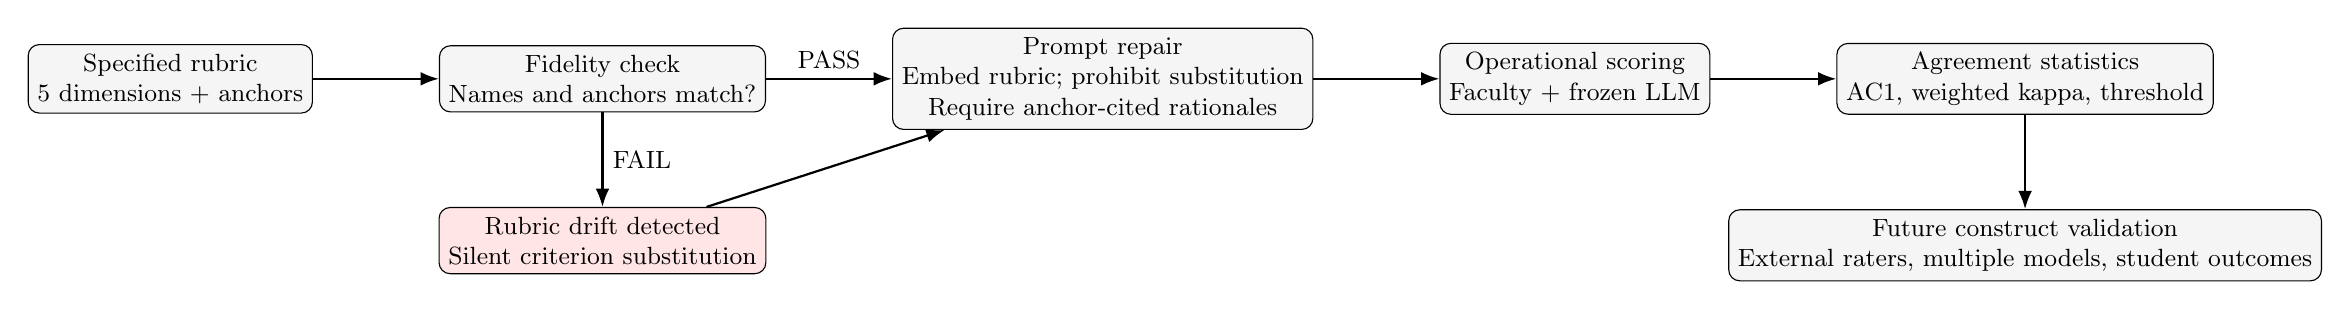
\begin{tikzpicture}[font=\small, node distance=1.2cm and 1.6cm, every node/.style={align=center}, box/.style={draw, rounded corners, minimum width=2.5cm, minimum height=.78cm, fill=gray!8}, warn/.style={draw, rounded corners, minimum width=2.5cm, minimum height=.78cm, fill=red!10}, arrow/.style={-Latex, thick}]
\node[box] (rubric) {Specified rubric\\5 dimensions + anchors};
\node[box, right=of rubric] (check) {Fidelity check\\Names and anchors match?};
\node[warn, below=of check] (drift) {Rubric drift detected\\Silent criterion substitution};
\node[box, right=of check] (repair) {Prompt repair\\Embed rubric; prohibit substitution\\Require anchor-cited rationales};
\node[box, right=of repair] (scoring) {Operational scoring\\Faculty + frozen LLM};
\node[box, right=of scoring] (stats) {Agreement statistics\\AC1, weighted kappa, threshold};
\node[box, below=of stats] (future) {Future construct validation\\External raters, multiple models, student outcomes};
\draw[arrow] (rubric) -- (check);
\draw[arrow] (check) -- node[above]{PASS} (repair);
\draw[arrow] (repair) -- (scoring);
\draw[arrow] (scoring) -- (stats);
\draw[arrow] (stats) -- (future);
\draw[arrow] (check) -- node[right]{FAIL} (drift);
\draw[arrow] (drift) -- (repair);
\end{tikzpicture}%
}
\caption{Prompt-fidelity workflow from rubric lock and runtime verification through operational agreement and future construct validation.}
\label{fig:workflow}
\end{figure*}

The repaired prompt used four linked safeguards: complete rubric embedding, explicit substitution prohibition, anchor-cited rationales, and runtime verification before and during scoring (Figure~\ref{fig:workflow}). The corrected evaluator named all five dimensions verbatim at both checks, and no further substitution appeared in the 10-prompt run. This does not prove that every possible fidelity failure was absent, but it directly controlled the documented failure mode.

\subsection{Faculty Agreement}
Across six faculty pairs and the four discriminating dimensions, mean AC1 was 0.287 and mean quadratic weighted kappa was 0.408. Pairwise AC1 ranged from -0.042 (95\% bootstrap CI [-0.308, 0.288]) to 0.532 [0.259, 0.799]. Including the floored Ethical GenAI Use dimension raises the five-dimension means to 0.451 and 0.485, an arithmetic effect of a dimension on which agreement is perfect by construction, not additional evidence of consistency. In practical terms, two faculty raters typically assigned the same or an adjacent score on a dimension, but matched exactly only somewhat more often than chance alone would produce, enough consistency to support screening, not enough to treat any single rater's scores as definitive. One rater scored all prompts at or below the operational keep boundary. Excluding that rater in a sensitivity analysis increased the four-dimension mean AC1 to 0.383 and weighted kappa to 0.499 (five-dimension basis: 0.522 and 0.575); the overall interpretation is fair-to-moderate agreement.

Disagreement was concentrated in applied labs and team projects, where total-score ranges reached 5 to 7 points after correction. Written assignments generally produced ranges of 1 to 2 points. Ethical GenAI Use showed the provenance floor anticipated in Section~\ref{sec:methods}: all 40 faculty ratings were 1, observed agreement and AC1 were 1.000, and quadratic weighted kappa was not estimable because all ratings occupied one category.

\subsection{LLM Agreement}
Over the four discriminating dimensions, pooled LLM-faculty AC1 averaged 0.216 and weighted kappa averaged 0.474, with pairwise AC1 ranging from 0.008 (95\% bootstrap CI [-0.190, 0.213]) to 0.450 [0.187, 0.713]. On the five-dimension basis the values are 0.388 and 0.573 (pairwise 0.230 to 0.559), inflated by the shared Ethical GenAI Use floor in the same way as the faculty statistics. Relative to the faculty benchmarks (AC1 = 0.287; kappa = 0.408), the model agreed with faculty roughly as well as faculty agreed with one another, slightly lower on exact matches, slightly higher on ordinal closeness. This comparability is evidence about agreement, not construct validity; faculty and model agreement can coexist with systematic limitations in how the intended educational construct is represented or scored. All 10 LLM Ethical GenAI Use ratings were 1; the dimension is excluded from the primary means and reported separately, since agreement at a uniform floor carries no discriminating information.

The LLM total exceeded the corrected faculty mean on 9 of 10 prompts. The largest gaps occurred on applied cases rather than hands-on labs. The direction suggests a modest positive scoring tendency, but the small sample does not support a stable bias estimate. More importantly, the model remained inside the intended rubric after the fidelity repair.

\subsection{Threshold Agreement}
At the published redesign boundary (total $<$ 10 = REVISE; total $\geq$ 10 = KEEP), faculty pairwise simple agreement ranged from 60\% to 100\% (dichotomized kappa 0.000 to 1.000), and LLM-faculty agreement from 70\% to 80\% (kappa -0.154 to 0.545). Two raters produced identical keep-or-revise decisions on all ten prompts; kappa collapsed to or below zero wherever one rater flagged nearly every prompt, leaving little marginal variation for chance correction. During verification, an Excel workbook instruction was found to contain a threshold wording error that stated totals of 10 and below should be revised. The published instrument stated below 10, so total scores of exactly 10 were analyzed as KEEP. The replication package documents the correction and preserves the raw workbook note. Threshold agreement was useful for screening, but insufficiently stable to support unsupervised keep-or-revise decisions.

\subsection{Summary}
\begin{table}[t]
\caption{Summary of pilot agreement results.}
\label{tab:summary}
\begin{tabular}{@{}p{0.46\linewidth}p{0.46\linewidth}@{}}
\toprule
Metric and estimate & Interpretation \\
\midrule
Faculty AC1: 0.287 (0.451 incl. floor dimension) & Fair-to-moderate consistency over dimensions with score variation. \\
Faculty kappa: 0.408 (0.485 incl. floor) & Fair-to-moderate ordinal agreement after data correction. \\
LLM AC1: 0.216 (0.388 incl. floor dimension) & Comparable to faculty values on both bases, with substantial pair variation. \\
LLM kappa: 0.474 (0.573 incl. floor) & Ordinal agreement slightly above the faculty mean after fidelity repair and score correction. \\
Threshold: faculty 60\%-100\%; LLM 70\%-80\% & Decision consistency varies too widely for autonomous use. \\
\bottomrule
\end{tabular}
\end{table}

Table~\ref{tab:summary} summarizes the findings. The floor dimension is disclosed for completeness but treated separately because it carries no discriminating evidence in this sample.

\section{Discussion}
\textbf{Implication 1: Prompt fidelity is a reportable method variable.} Model name, temperature, and prompt text are not enough. Researchers should demonstrate that the model retained the intended rubric at the point of scoring. A preflight dimension check and at least one in-run check are inexpensive controls against a failure that otherwise leaves plausible-looking data. This failure class is not idiosyncratic to one session or model: concurrent work documents rubric instability under nominally fixed prompts and systematic vulnerabilities in LLM judges \cite{hong2026rubrics,thakur2025judging}. Studies that reference an external rubric without embedding and verifying it should be interpreted cautiously.

\textbf{Implication 2: Reliability statistics require a fidelity gate.} The correct workflow is fidelity verification, then operational agreement, and only then validity research. A coefficient can be computed on any two numeric columns, but it is methodologically meaningless when one evaluator scored a substituted construct. The gate matters most in automated pipelines, where large volumes of scores can be produced before a human inspects criterion-level output.

\textbf{Implication 3: LLMs can support triage, but faculty remain accountable.} After repair, LLM-faculty agreement was within the range of faculty-faculty agreement. That finding supports a bounded use case: the model can flag prompts, surface missing design elements, and provide a contrasting rationale for faculty review. It does not justify autonomous redesign decisions. The LLM was somewhat more generous than the faculty mean, threshold agreement varied, and faculty themselves diverged most on complex labs and team projects. Human review is most necessary precisely where contextual teaching knowledge is least visible in the prompt.

\textbf{Implication 4: The next study must target discriminating evidence.} Because every sampled prompt predated GenAI-era design expectations, a score of 1 on Ethical GenAI Use was the historically appropriate rating, and the dimension had no opportunity to discriminate. A larger validation should stratify prompts by original publication and revision date, deliberately include GenAI-era assignments, include external non-author raters, randomize or counterbalance order, compare additional models, and archive raw model outputs.

\section{Limitations}
\label{sec:limitations}
This exploratory pilot used 10 assignments, one institution's four co-author raters, one hosted model, and one scoring period. The small stratified sample supports demonstration and initial testing of the workflow but does not establish robustness, transferability, or stable subgroup effects. Co-author raters may share assumptions despite independent scoring, and faculty order was not randomized. Only public prompt text was scored, not surrounding instruction or student performance. The Ethical GenAI Use floor was structurally induced by a pre-GenAI sample. Model decoding and retention settings were requested through the institutional interface rather than independently verified; the university's non-API configuration exposes no endpoint controls, so verified determinism, the ideal, was not attainable in this study, and hosted-model behavior may change over time. The corrected prompt reduced observed rubric substitution risk but cannot exclude other prompt-fidelity failures. Finally, operational agreement is not construct validation; the relationship between rubric scores, student learning, authorship evidence, and assessment consequences remains untested.

\section{Conclusion}
This pilot's most consequential result occurred before any agreement analysis: an LLM evaluator silently replaced the intended five-dimension rubric while returning persuasive, correctly formatted output. Drift of this kind is widely experienced and tolerated in everyday LLM use; rubric-based assessment cannot tolerate it, and must prevent it by overt prompt design. Embedding the complete rubric, prohibiting substitution, requiring anchor-cited rationales, and verifying the dimension set at runtime restored fidelity and made the subsequent statistics interpretable. After correction, faculty-faculty agreement over the dimensions with score variation was fair to moderate (mean AC1 = 0.287; 0.451 when the floored dimension is included) and LLM-faculty agreement was comparable (four-dimension mean AC1 = 0.216; five-dimension 0.388), while keep-or-revise decisions varied too widely for autonomous use. The defensible near-term role for the model is a disclosed second reader that helps faculty identify assignment prompts for review while preserving human accountability. Future work should test these safeguards across models and institutions, recruit independent raters, and connect prompt-level scores to student evidence. LLM-as-judge studies should report prompt-fidelity verification alongside model version, prompting strategy, and inter-rater agreement as standard methodological transparency.

\ifanonymousreview
% Acknowledgments are omitted during anonymous review.
\else
\section*{Acknowledgments}
The authors thank the CLARK Cybersecurity Curriculum Library and SEED Labs for maintaining openly available instructional resources.
\fi

\section*{Supplementary Materials}
The public replication package is available at \url{https://github.com/01OrangeCrush/DREAM-II}. It includes the frozen evaluator prompt, drift episode transcript, fidelity verification transcripts, sample catalog with source links and licenses, seeded randomization key, de-identified scoring data and correction log, analysis scripts, and model documentation.


\begin{thebibliography}{18}

\bibitem{akbar2025beyond}
Muhammad Sajjad Akbar. 2025. Beyond detection: Designing AI-resilient assessments with automated feedback tool to foster critical thinking and originality. \emph{arXiv preprint arXiv:2503.23622}. https://doi.org/10.48550/arXiv.2503.23622

\bibitem{cohen1968weighted}
Jacob Cohen. 1968. Weighted kappa: Nominal scale agreement provision for scaled disagreement or partial credit. \emph{Psychological Bulletin} 70, 4 (1968), 213--220. https://doi.org/10.1037/h0026256

\bibitem{feinstein1990high}
Alvan R. Feinstein and Domenic V. Cicchetti. 1990. High agreement but low kappa: I. The problems of two paradoxes. \emph{Journal of Clinical Epidemiology} 43, 6 (1990), 543--549. https://doi.org/10.1016/0895-4356(90)90158-L

\bibitem{fowler2023ai}
David S. Fowler. 2023. AI in higher education: Academic integrity, harmony of insights, and recommendations. \emph{Journal of Ethics in Higher Education} 3 (2023), 127--143. https://doi.org/10.26034/fr.jehe.2023.4657

\bibitem{gwet2008computing}
Kilem Li Gwet. 2008. Computing inter-rater reliability and its variance in the presence of high agreement. \emph{British Journal of Mathematical and Statistical Psychology} 61, 1 (2008), 29--48. https://doi.org/10.1348/000711006X126600

\bibitem{hong2026rubrics}
Yihan Hong, Huaiyuan Yao, Bolin Shen, Wanpeng Xu, Hua Wei, and Yushun Dong. 2026. From rubrics to reliable scores: Evidence-grounded text evaluation with LLM judges. \emph{arXiv preprint arXiv:2601.08654}. https://doi.org/10.48550/arXiv.2601.08654

\bibitem{jongkind2026curriculum}
Remco Jongkind, Erik Elings, Erik Joukes, Tom Broens, Henrik Leopold, Floris Wiesman, and Jelle Meinema. 2026. Is your curriculum GenAI-proof? A method for GenAI impact assessment and a case study (Version 3). \emph{MedEdPublish} 15, 11. https://doi.org/10.12688/mep.20815.3

\bibitem{liu2023geval}
Yang Liu, Dan Iter, Yichong Xu, Shuohang Wang, Ruochen Xu, and Chenguang Zhu. 2023. G-Eval: NLG evaluation using GPT-4 with better human alignment. In \emph{Proceedings of the 2023 Conference on Empirical Methods in Natural Language Processing}. Association for Computational Linguistics, Singapore, 2511--2522. https://doi.org/10.18653/v1/2023.emnlp-main.153

\bibitem{mccauley2025undergraduate}
Jennifer McCauley, Edward J. Glantz, Mahdi Nasereddin, and Michael R. Bartolacci. 2025. Undergraduate cybersecurity redesign for the GenAI era: Beyond authentic assessment. In \emph{Proceedings of the 26th ACM Annual Conference on Cybersecurity and Information Technology Education (SIGCITE '25)}. Association for Computing Machinery, New York, NY, USA, 47--51. https://doi.org/10.1145/3769694.3771116

\bibitem{messick1995validity}
Samuel Messick. 1995. Validity of psychological assessment: Validation of inferences from persons' responses and performances as scientific inquiry into score meaning. \emph{American Psychologist} 50, 9 (1995), 741--749. https://doi.org/10.1037/0003-066X.50.9.741

\bibitem{miao2023guidance}
Fengchun Miao and Wayne Holmes. 2023. \emph{Guidance for Generative AI in Education and Research}. UNESCO, Paris. https://doi.org/10.54675/EWZM9535

\bibitem{peng2026dimension}
Gang Peng. 2026. Dimension-level intent fidelity evaluation for large language models: Evidence from structured prompt ablation. \emph{arXiv preprint arXiv:2605.14517}. https://doi.org/10.48550/arXiv.2605.14517

\bibitem{powell2024generative}
Stephen Powell and Rachel Forsyth. 2024. Generative AI and the implications for authentic assessment. In Sue Beckingham, Jenny Lawrence, Stephen Powell, and Peter Hartley (Eds.), \emph{Using Generative AI Effectively in Higher Education}. Routledge, London, 97--105. https://doi.org/10.4324/9781003482918-15

\bibitem{rhodes2013value}
Terrel L. Rhodes and Ashley Finley. 2013. \emph{Using the VALUE Rubrics for Improvement of Learning and Authentic Assessment}. Association of American Colleges and Universities, Washington, DC. https://www.aacu.org/publication/using-the-value-rubrics-for-improvement-of-learning-and-authentic-assessment

\bibitem{shneiderman2022human}
Ben Shneiderman. 2022. \emph{Human-Centered AI}. Oxford University Press, Oxford. https://doi.org/10.1093/oso/9780192845290.001.0001

\bibitem{szafran2017miscalculation}
Robert Szafran. 2017. The miscalculation of interrater reliability: A case study involving the AAC\&U VALUE rubrics. \emph{Practical Assessment, Research, and Evaluation} 22, 1 (2017), Article 11. https://doi.org/10.7275/xfp0-8228

\bibitem{thakur2025judging}
Aman Singh Thakur, Kartik Choudhary, Venkat Srinik Ramayapally, Sankaran Vaidyanathan, and Dieuwke Hupkes. 2025. Judging the judges: Evaluating alignment and vulnerabilities in LLMs-as-judges. In \emph{Proceedings of the Fourth Workshop on Generation, Evaluation and Metrics}. Association for Computational Linguistics, Vienna, Austria, 404--430. https://aclanthology.org/2025.gem-1.33/

\bibitem{zheng2023judging}
Lianmin Zheng, Wei-Lin Chiang, Ying Sheng, Siyuan Zhuang, Zhanghao Wu, Yonghao Zhuang, Zi Lin, Zhuohan Li, Dacheng Li, Eric P. Xing, Hao Zhang, Joseph E. Gonzalez, and Ion Stoica. 2023. Judging LLM-as-a-judge with MT-Bench and Chatbot Arena. In \emph{Advances in Neural Information Processing Systems 36}. 46595--46623. https://arxiv.org/abs/2306.05685

\end{thebibliography}

\end{document}
